\documentclass[twocolumn,aps,prb,citeautoscript]{revtex4-1}
\usepackage{graphicx}

\begin{document}

\title{Summer Undergraduate Research Fellowship Proposal:\\
Effects of superconducting lead endcaps on boundary conditions of
magnetic fields}
\author{Aritra Biswas, with Filippone Group}
\affiliation{W.K. Kellogg Radiation
Laboratory, California Institute of Technology}

%\begin{abstract}

%\end{abstract}

\maketitle

\section{Motivation}
The discovery of charge-parity symmetry (CP) violation 
in the decay of neutral kaons has incited various attempts to extend the
Standard Model to explain CP violation \cite{cpv}. Measurements of the electric
dipole moments of various particles provide important restrictions on these
attempts and could guide reformulations of the Standard Model \cite{ill}.

In particular, previous efforts \cite{ill} to determine the electric dipole
moment  of the neutron (nEDM)
have yielded a numerical limit of $|d_n| < 2.9 \times 10^{-26}e\text{ cm}$.
The nEDM collaboration intends to
improve this limit \cite{krl} by measuring the behavior of trapped
ultra-cold neutrons (UCN) in a magnetic field.
The experiment is currently being modeled at
half-scale at Caltech.

Determining the nEDM involves observing neutron movement in a magnetic field
that must be uniform; if not, a
``geometric phase effect'' creates the same shift in Larmor precession
that would be measured if there were an EDM, thus creating the semblance
of a false EDM\cite{coil}.
The primarily experimental challenge is to create a contained magnetic field
that can be controlled to point uniformly along a specific direction. To
eliminate
the influence of the Earth's field and other interference, and to contain
the field, the setup is surrounded by a cylindrical
superconducting lead shield. While
this method shields the center of the experimental setup well,
it can create undesired behavior
in the magnetic field profile at the circular faces of the cylinder, which
were previously not covered with superconducting material.

We plan to cover the faces of the cylinder with superconducting lead endcaps
to create favorable boundary conditions for the magnetic field.
While various styles of bridging the gap between the cylinder and the endcaps
for the nEDM experiment have
been explored \cite{endcapstyles}, further measurements are required to
determine the effects of these endcaps on the boundary conditions of
the magnetic field.

A fuller understanding of these effects is critical to
controlling the magnetic field and addressing potential challenges in the
final nEDM experiment before they arise. 

\begin{figure}
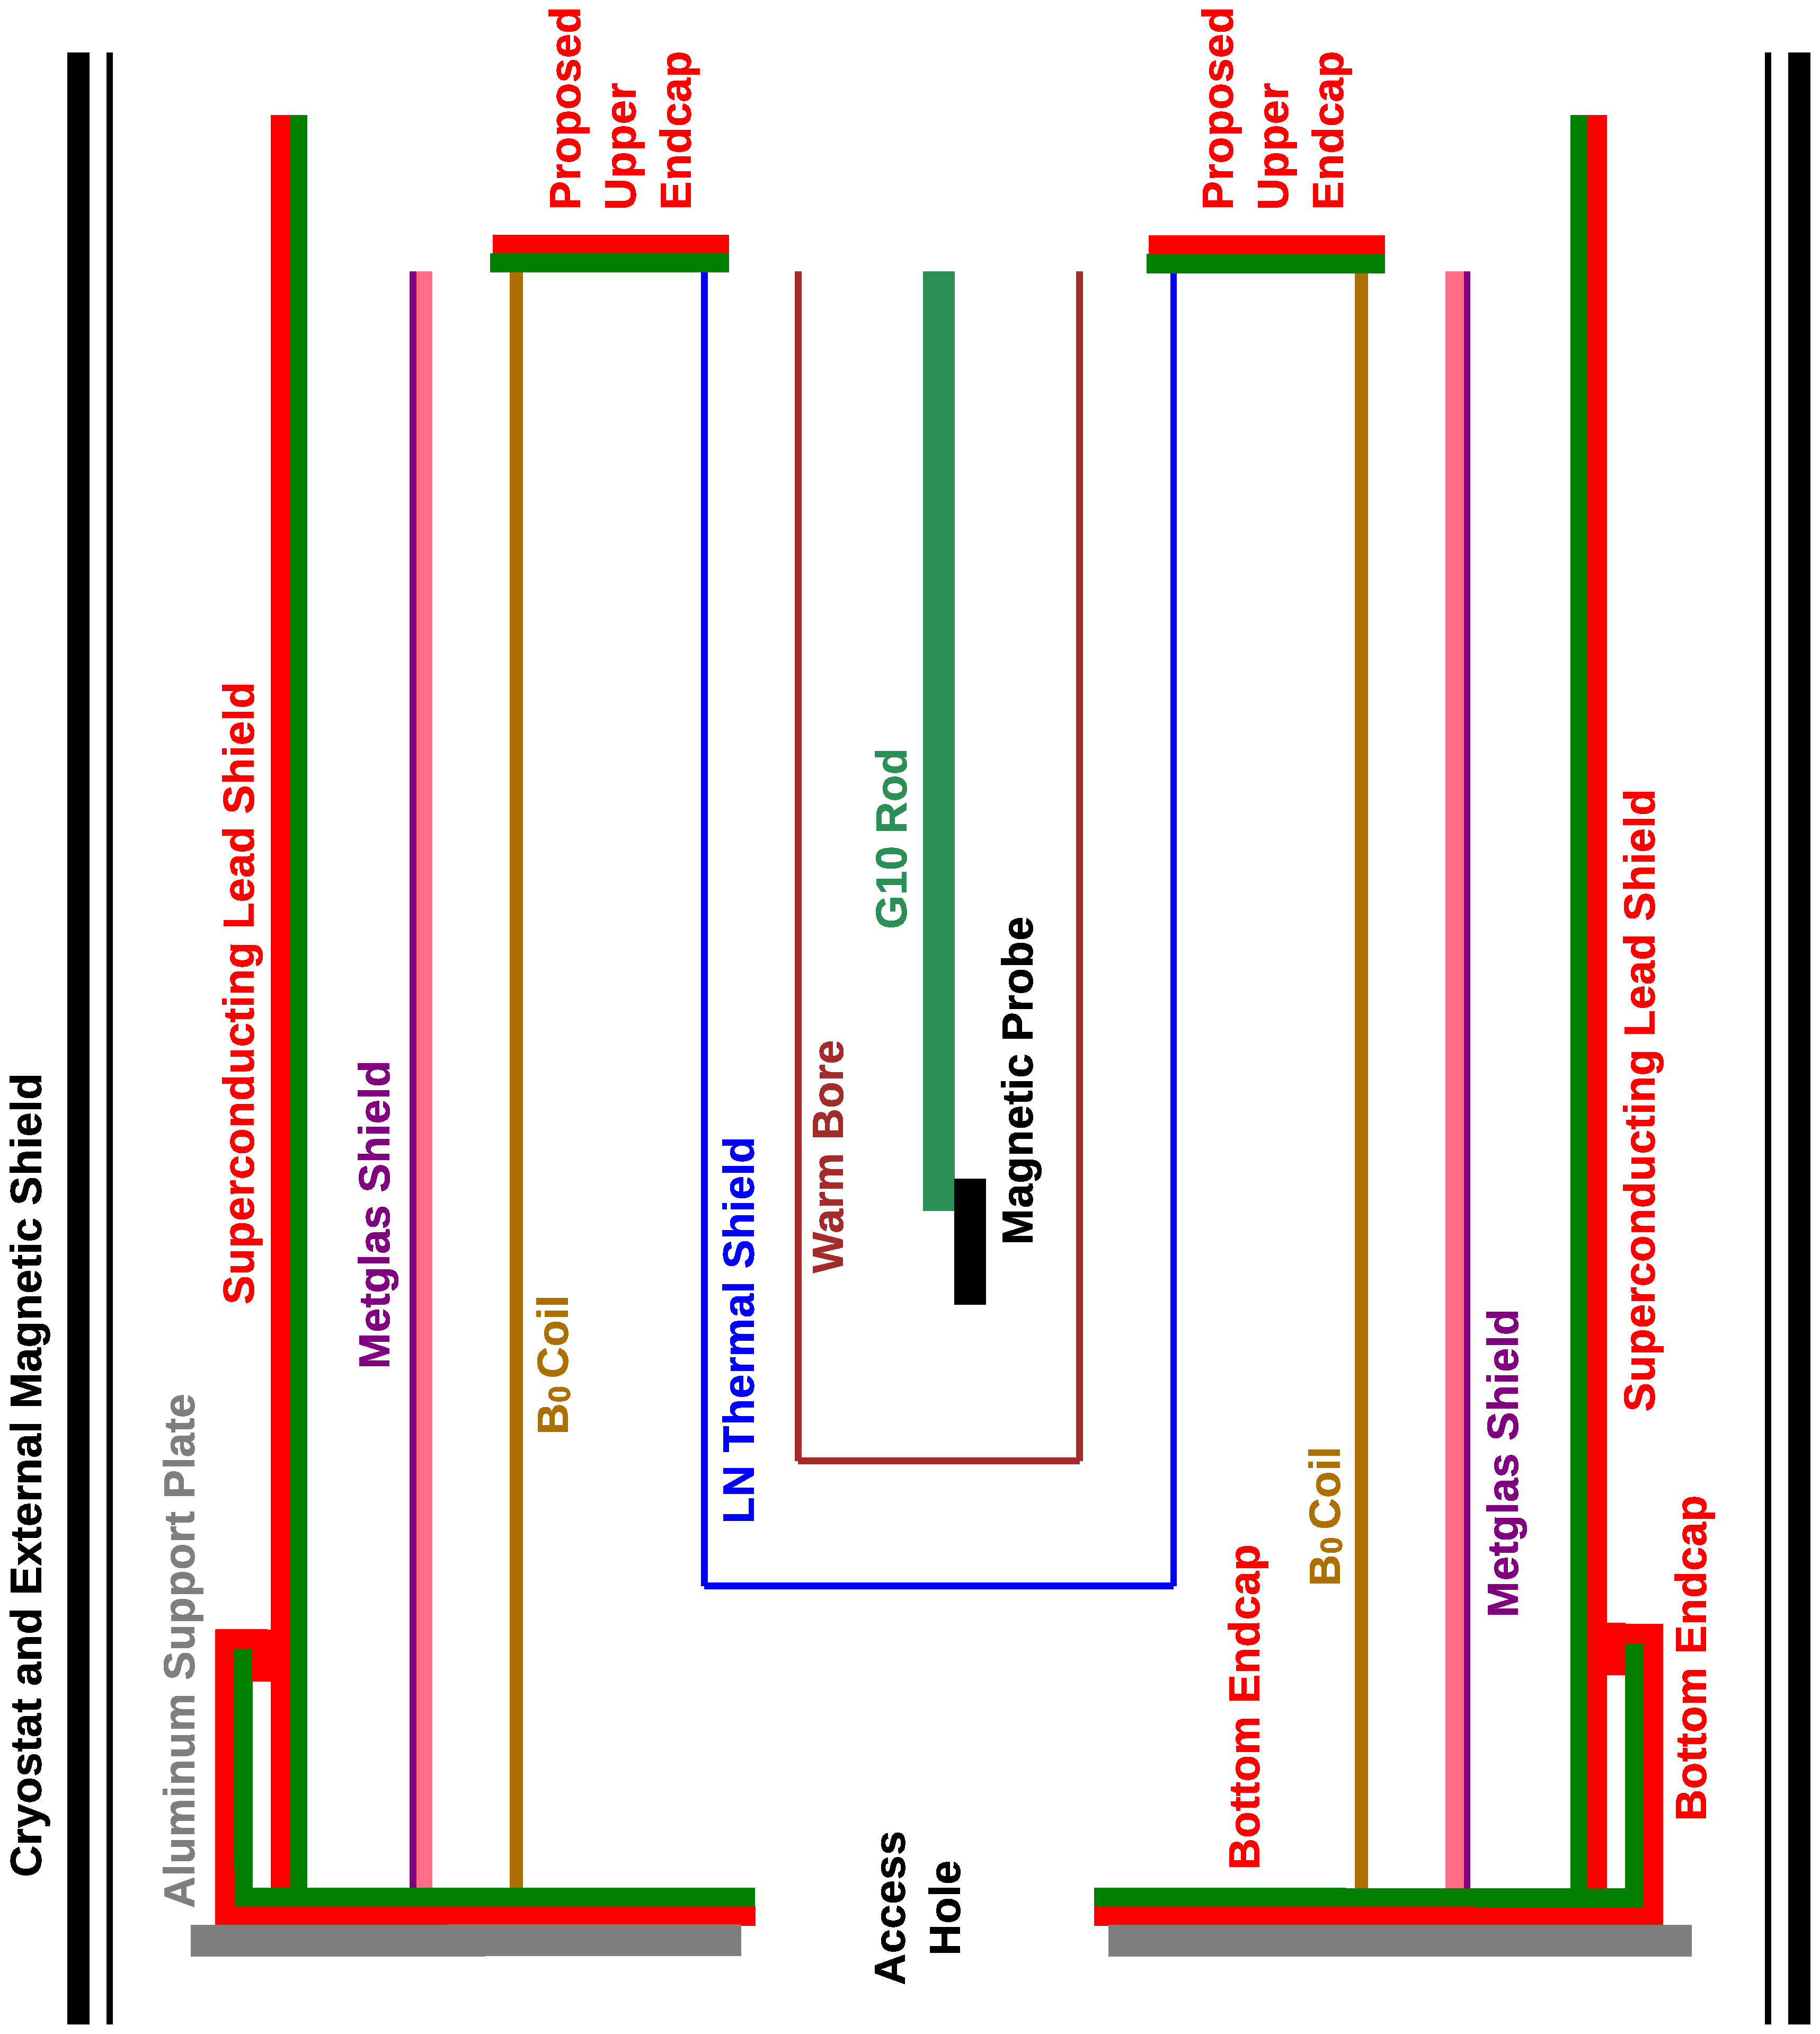
\includegraphics[width=0.45\textwidth]{out.eps}
\caption{\label{fig:structure}Stylized diagram of the experimental
setup.}
\end{figure}

\section{Experimental Setup}

The half-scale model magnet model at Caltech, shown in
Figure \ref{fig:structure}, consists of various
cylindrical
shells placed inside each other. The innermost structure is 
a G-10 plastic rod holding a 3-axis magnetic probe; these are encircled by a
warm bore cylinder and a liquid nitrogen thermal shield.

Surrounding this foil is
an acrylic structure with various coils of wire arranged in a $\cos\theta$ coil
geometry
to approximate a sheet current and produce the desired magnetic field
profile \cite{coil}.
These coils are collectively referred
to as the $B_0$ coil.

Each individual current in the $B_0$ coil, including shimming coils
necessary for correcting non-uniformities in the field \cite{coil}, is
controlled through a NI LabView Virtual Instrument (VI).

The $B_0$ coil is covered by a cylindrical Metglas 2705M magnetic
alloy which serves to redirect the horizontal magnetic field from the $B_0$
coil vertically along the surface of the Metglas. Surrounding this layer is the
the superconducting lead cylinder, to which the endcaps in
question will be attached. The external cryostat shield surrounds this
structure.

The bottom endcap is a G-10 annulus with a
wall along the outer edge; this forms a ``cup'' shape with an access hole
at the bottom. A lead sheet is fitted along the underside of
the annulus and around the outside face of the wall, creating an enclosure
over the top of the wall. The top endcap, while designed, has not yet been
installed.

Along the lead shield are several helium cooling lines. While there are no
cooling lines directly on the bottom endcap, the endcap sits on an aluminum
plate which has cooling lines underneath it. This aluminum plate serves
as a base for the entire setup and bears the weight of the $B_0$ coil, the
Metglas shield, the lead shield, and the bottom endcap
(totaling approximately 500 lbs), and will also cool
the bottom endcap by contact.

Temperature probes are installed at various points, including on the $B_0$
coil, on multiple areas of the lead shield, and on multiple areas of the
bottom lead endcap. Lakeshore DT670 silicon diode temperature sensors are
used on the endcap.

\begin{figure}
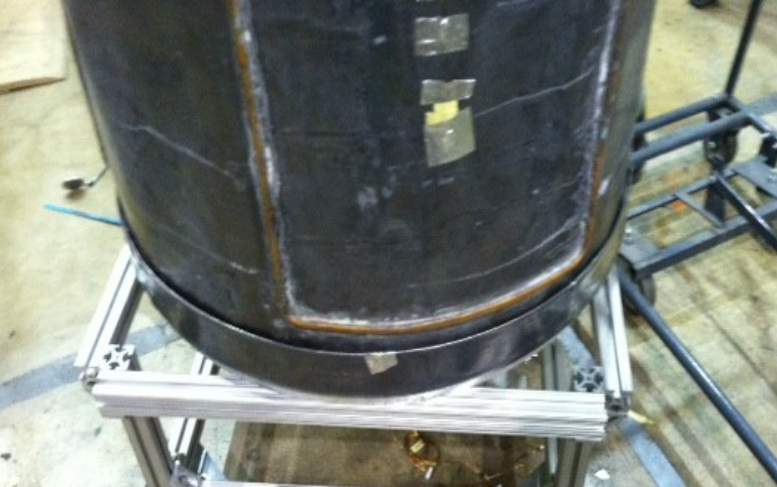
\includegraphics[width=0.45\textwidth]{endcap.png}
\caption{\label{fig:endcap}The lead shield and the attached bottom endcap.}
\end{figure}

\section{Procedure and Measurements}

Over several hours, the cryostat will be evacuated for thermal insulation and
the cooling lines will bring the lead shield to below superconducting
temperature (4 K).

To assess the effectiveness of the bottom endcap design, we will
measure its temperature over time. Although contact cooling in a vaccuum
is difficult, because of the 500 pounds of normal force between the
cooled aluminum plate and the lead endcap, we expect the thermal contact to be
sufficient to bring the lead endcap to the desired superconducting
temperature. If the contact is unsuitable, we will explore alternatives such as
improving the contact surface with thermal grease or considering alternative
endcap designs where the endcap is cooled directly. 

We will conduct measurements of the magnetic field gradient
at multiple points near the bottom endcap and compare these
gradients with measurements obtained from the center of the apparatus
and with previous measurements taken before the endcap was installed. These
gradient comparisons will allow us to determine the general effectiveness of
the endcap in generating favorable boundary conditions (uniformity of the
field); in addition, they will provide an additional method to ensure that the
bottom endcap is indeed superconducting.

The collection of magnetic probe data
is carried out in another LabView VI. Data is collected
for the magnetic fields along three axes to create $B_x, B_y,$ and $B_z$
arrays, each of which are plotted along the three spatial axes to create nine
waveform graphs. We plan to analyze this data and create a model of the
magnetic field behavior near the endcap compared to its behavior in other parts
of the setup.

After examining the results, we will consider the effectiveness of the current
endcap design, which could prompt modifications. Measurements
will be repeated for the top endcap once it is installed
to create a comprehensive profile of
the changes caused by these endcaps in the boundary conditions of the field.

\section{Personal Work Status}

Since November 2013, my work in this experiment has involved:
\begin{itemize}
\item editing and developing the LabView VI used for field monitoring and
shimming to synchronize magnetic field measurement sampling rates,
\item developing tools, including a new VI, to compare magnetic field mapping
data from various runs, and
\item assisting with the installation of the bottom endcap and re-assembly
of the setup, including reconfiguring temperature sensors.
\end{itemize}

A potential checklist for the summer will include:
\begin{itemize}
\item finishing the development of the aforementioned tools necessary to
compare magnetic fields mappings,
\item assessing the effectiveness of the thermal contact between the bottom
endcap and the support plate,
\item comparing the magnetic field profiles at the boundary near the installed
endcap vs. at the center of the $B_0$ coil,
\item comparing the magnetic field profile of the post-endcap setup vs. the
previous setup,
\item assisting with the construction of a top endcap, its installation, and
re-assembly of the setup,
\item repeating magnetic field comparisons for the top endcap, and
\item developing numerical data analysis tools as necessary.
\end{itemize}

These steps lead to a better understanding of the effect of
superconducting endcaps on the magnetic field in our model. The
results will be key to the planning of the nEDM experiment and could prove
useful to other particle physics experiments using similar superconducting
endcaps.

\begin{thebibliography}{}
\bibitem{cpv} Cronin, J. ``Nobel Lecture: CP Symmetry Violation – The Search
for Its Origin,'' Nobel Media AB (2013).
\bibitem{ill} Baker, C. A., D. D. Doyle, P. Geltenbort, K. Green, M. G. D. Van der Grinten, P. G. Harris, P. Iaydjiev et al. ``Improved experimental limit on the electric dipole moment of the neutron.'' \textit{Physical Review Letters} 97, no. 13 (2006): 131801.
\bibitem{krl} ``Search for the nEDM at Caltech.'' Kellogg Radiation Laboratory
$\langle$krl.caltech.edu$\rangle$ (2014).
\bibitem{endcapstyles} Malkowski, S., R. Y. Adhikari, J. Boissevain, C. Daurer, B. W. Filippone, B. Hona, B. Plaster, D. Woods, and H. Yan. ``Overlap Technique for End-Cap Seals on Cylindrical Magnetic Shields.'' \textit{IEEE Transactions on Magnetics} 49, no. 1 (2013): 651-653.
\bibitem{coil} Perez Galvan, A., B. Plaster, J. Boissevain, R. Carr, B. W. Filippone, M. P. Mendenhall, R. Schmid, R. Alarcon, and S. Balascuta. ``High uniformity magnetic coil for search of neutron electric dipole moment.'' \textit{Nuclear Instruments and Methods in Physics Research Section A: Accelerators, Spectrometers, Detectors and Associated Equipment} 660, no. 1 (2011): 147-153.
\end{thebibliography}

\end{document}
